\chapter{Stage 02: Earth Engine export and image processing}
\label{ch:stage02}

Stage~02 turns five global datasets into a neat package for each patch. It has two halves: \textbf{export} in Google Earth Engine \citep{gorelick2017} (notebook 01) and \textbf{digital image processing}, or DIP, on your computer (notebook 02).

\section{The candidate pool}

\file{data/raw_metadata/composite_stats.csv} holds \textbf{1,200 candidate patches}, each with Earth Engine statistics: index means for both years, radar means, climate values, terrain, masked fraction and the changes (for example \texttt{ndvi\_change}). The pool was made in an earlier (``parent'') repository and copied in. All candidate centres lie inside the study rectangle.

\begin{figure}[H]
\centering
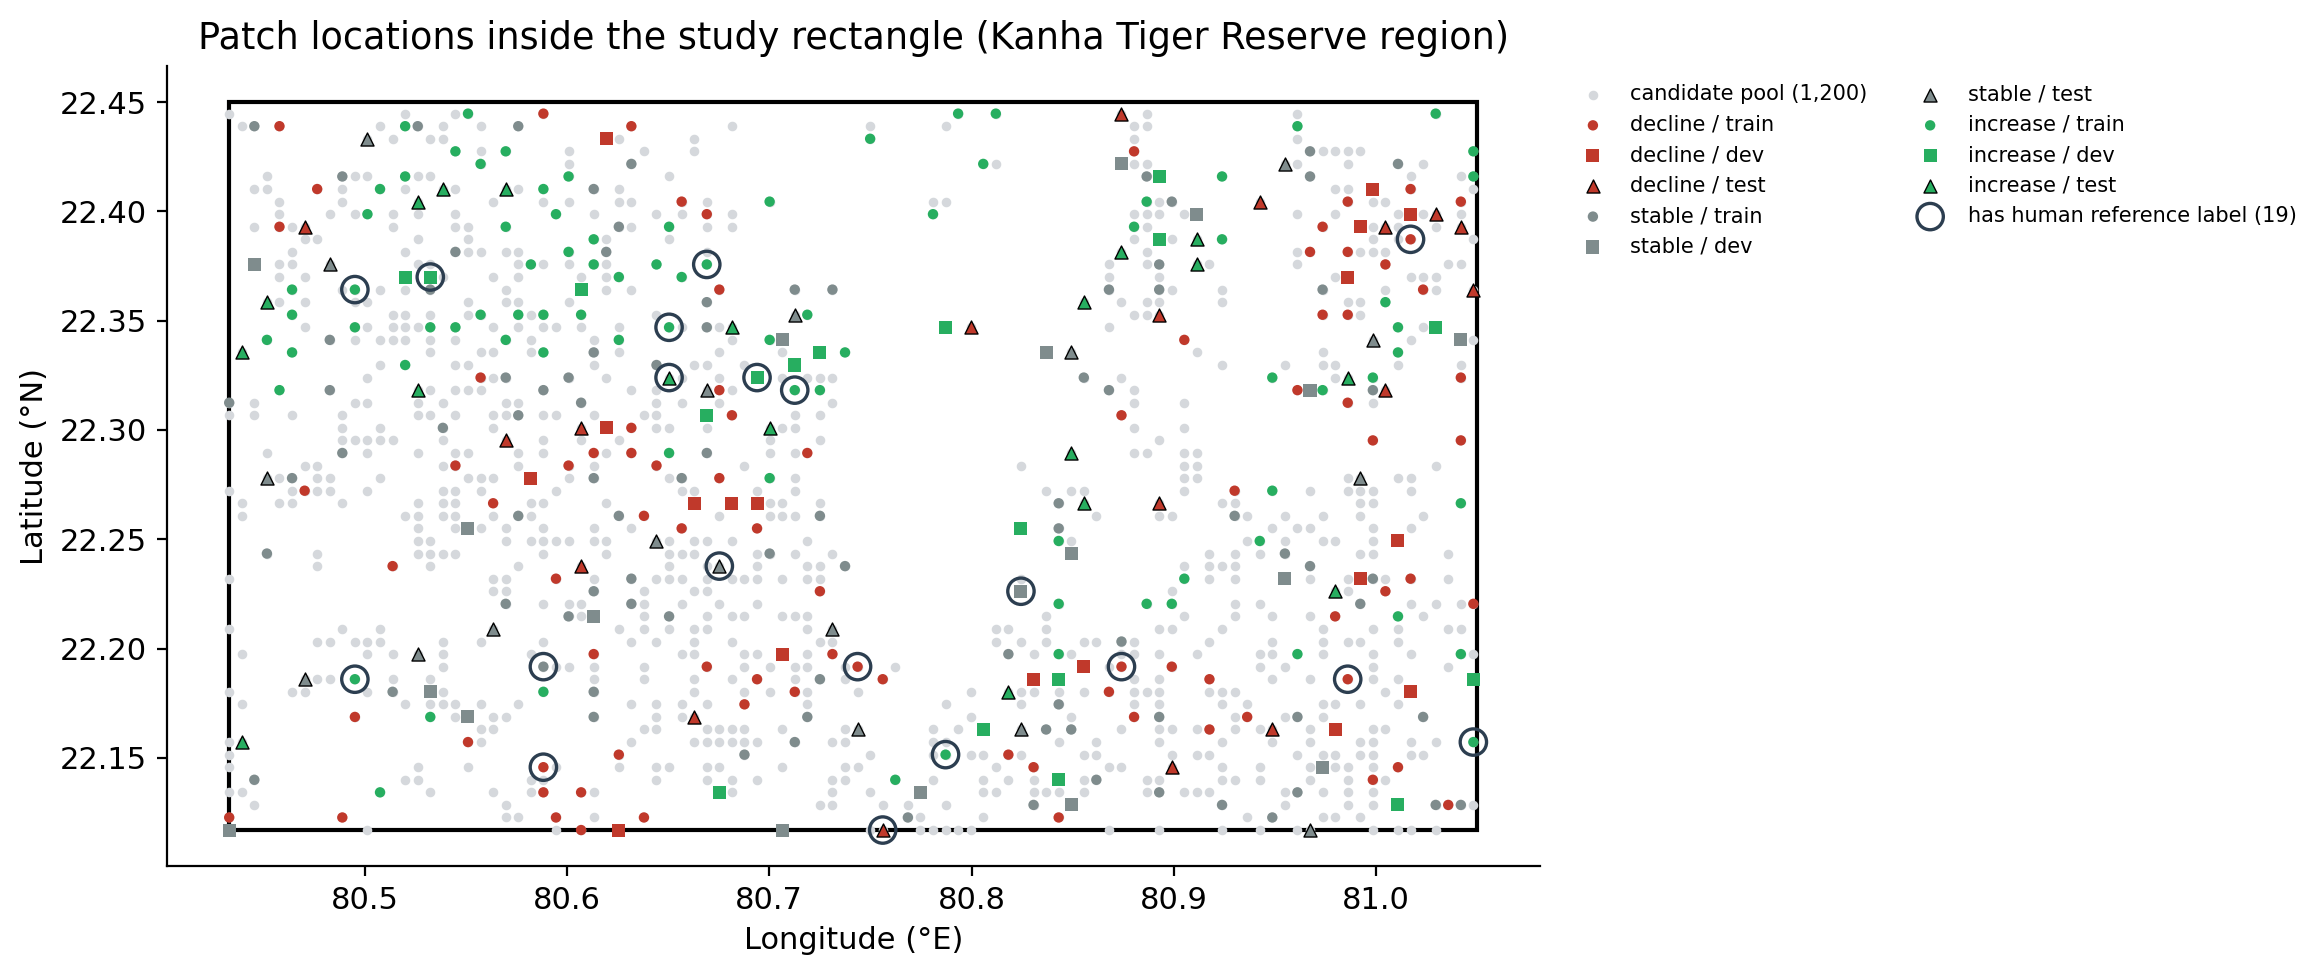
\includegraphics[width=\textwidth]{figures/fig_patch_map.png}
\caption{All 1,200 candidate centres (grey) and the 366 selected patches, coloured by class, with marker shape showing the split. Circles mark the 19 patches with a human label. Made by \file{study_guide/make_figures.py} from \file{data/raw_metadata/}.}
\label{fig:patchmap}
\end{figure}

\begin{watchout}
The pool has an empty vertical strip near 80.75--80.85\dg E (Figure~\ref{fig:patchmap}). The parent repository does not record why. The most likely reason is a forest-cover filter (for example, farmland or a valley without forest), but you do not know this. In the report, describe the strip and say the reason was not recorded; do not invent one.
\end{watchout}

\section{Patch geometry}

Each patch is built around its centre point (\texttt{patch\_geometry}): a circle of radius 320\,m is drawn (half of $64 \times 10$\,m), its bounding square is taken, and the square is intersected with the study rectangle. So a patch is a square of about 640\,m, and patches on the edge of the rectangle are cut short.

\begin{watchout}
The export did not set a projected coordinate system, so Earth Engine used EPSG:4326 (degrees). One pixel is 0.0000898\dg, which is 10.0\,m north--south but only about 9.3\,m east--west at 22\dg N, because lines of longitude converge. The planned 64\,$\times$\,64 patches therefore came out as about 70\,$\times$\,65 pixels (302 of 366 patches; another 50 are 69\,$\times$\,65), and edge patches are smaller (p00052 is 70\,$\times$\,30). Nothing breaks, but if you write ``64\,$\times$\,64 pixels'' add ``about 640\,m, exported in geographic coordinates''.
\end{watchout}

\section{The export}

\begin{wherecode}
Notebook \file{notebooks/01_gee_extraction.ipynb} (the version actually run) and \file{scripts/01_export_gee.py}; helpers in \file{src/gee_utils.py} and \file{src/export_utils.py}.
\end{wherecode}

\begin{enumerate}
  \item Earth Engine builds every composite \emph{once} for the whole rectangle: Sentinel-2 medians for T0 and T1, Sentinel-1 medians (descending), CHIRPS totals, ERA5-Land anomalies, NASADEM terrain, the true-colour images, and \dndvi{} and \dnbr.
  \item For each patch, every layer is clipped to the patch square and downloaded with \texttt{geemap.ee\_export\_image} straight into \file{data/raw_tiffs/}.
  \item Work runs in batches of 100 with a log (\file{data/raw_metadata/local_export_log.txt}) and a state file, so a crash can resume without downloading everything again.
\end{enumerate}

\begin{table}[H]
\centering
\caption{The 15 GeoTIFFs exported per patch (\texttt{PATCH\_SUFFIXES} in \file{src/export_utils.py}); 5,490 files for 366 patches.}
\label{tab:15files}
\small
\begin{tabular}{lll}
\toprule
File suffix & Content & Typical size (pixels) \\
\midrule
\texttt{\_T0\_rgb}, \texttt{\_T1\_rgb} & B4, B3, B2 as reflectance (0--1) & 70\,$\times$\,65 \\
\texttt{\_T0\_s2\_optical}, \texttt{\_T1\_s2\_optical} & the 10 Sentinel-2 bands & 70\,$\times$\,65 \\
\texttt{\_T0\_indices}, \texttt{\_T1\_indices} & NDVI, EVI, NDMI, NBR & 70\,$\times$\,65 \\
\texttt{\_T0\_s1}, \texttt{\_T1\_s1} & VV, VH (dB) & 70\,$\times$\,65 \\
\texttt{\_T0\_rainfall}, \texttt{\_T1\_rainfall} & CHIRPS total (mm) & 1\,$\times$\,1 \\
\texttt{\_T0\_era5}, \texttt{\_T1\_era5} & temperature and soil-moisture anomalies & 1\,$\times$\,1 \\
\texttt{\_dem} & elevation, slope, aspect & about 24\,$\times$\,22 \\
\texttt{\_delta\_ndvi}, \texttt{\_delta\_nbr} & T1 $-$ T0 change & 70\,$\times$\,65 \\
\bottomrule
\end{tabular}
\end{table}

\begin{whybox}
Local download with \texttt{geemap} is faster than Earth Engine's ``export to Google Drive'' for small images; the Drive route stays as a fallback (\texttt{mode: drive} in the config, \file{scripts/02_download_drive.py}). Keeping all 15 layers, not only the colour images, means later experiments need no new download.
\end{whybox}

\subsection{Missing data}

Candidates whose masked fraction was above 0.15 (15\,\%) in either year were labelled ``uncertain'' and never sampled. For the 366 selected patches the masked fraction is between 0.8\,\% and 2.3\,\% (\file{data/raw_metadata/selected_patches.csv}).

\begin{watchout}
\texttt{masked\_frac\_before} and \texttt{masked\_frac\_after} are identical for all 366 patches. Real cloud masks for two different years would differ, so this value probably measures pixels lost at patch edges, not cloud. Describe it as ``very little missing data'', not as a measured cloud fraction.
\end{watchout}

\section{Image processing (DIP)}

Notebook \file{02_dip_auto_classify.ipynb} (``DIP + five-source packaging'') prepares what the models will see.

\subsection{Making the colour images look right}

Reflectance values of forest are small (about 0.02--0.1 in visible light), so they must be \emph{stretched} to the 0--255 display range. The first version stretched each band separately using percentiles. On small, dark forest chips this exaggerated noise and shifted the colours, producing purple images (Figure~\ref{fig:purple}). The fix was a fixed window: divide every band by 0.22 and clip to $[0, 1]$ (\texttt{percentile\_stretch\_rgb} in \file{src/dip_utils.py}, \texttt{vmax=0.22}), the same as the common Earth Engine display setting \texttt{min: 0, max: 2200}. It keeps the relative colours of the three bands, so forest looks green-brown.

\begin{figure}[H]
\centering
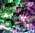
\includegraphics[width=0.22\textwidth]{figures/fig_purple.jpg}\hspace{1cm}
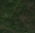
\includegraphics[width=0.22\textwidth]{figures/fig_natural.jpg}
\caption{The same chip with the first per-band stretch (left, purple) and with the fixed reflectance window used in the final pipeline (right). From \file{slides/figures/}.}
\label{fig:purple}
\end{figure}

\subsection{Padding and resizing to a 512\,$\times$\,512 canvas}

Vision--language models expect square images, and one canvas size lets every layer share the same coordinates (\texttt{pad\_and\_resize}):
\begin{enumerate}
  \item \textbf{Pad to a square} with zeros, split between both sides. A 65\,$\times$\,70 chip gets 5 rows of black.
  \item \textbf{Resize} the square to 512\,$\times$\,512: bilinear interpolation for colour images (smooth), nearest-neighbour for single-band arrays (keeps the original values).
  \item \textbf{Move any boxes} with the image: $x' = (x + p_x)\,s$, $y' = (y + p_y)\,s$, with $s = 512/\max(H, W)$ and $p_x, p_y$ the left and top padding.
\end{enumerate}

\begin{watchout}
Two consequences come back later.
\begin{enumerate}
  \item \textbf{No new detail.} Enlarging a 70-pixel chip to 512 pixels (about 7.3 times) only makes each pixel a bigger block. On the laptop the images were then shrunk again (longer side at most 336 pixels).
  \item \textbf{Padding enters the averages.} The arrays of indices and radar values are padded with 0, and the evidence card later averages the whole 512\,$\times$\,512 canvas, zeros included. For a 65-row chip padded to 70 rows, every mean is multiplied by about $65/70 = 0.93$; for the edge patch p00052 (30 rows) by about $30/70 = 0.43$. Chapter~\ref{ch:stage03} shows the effect on the card (the ``padding bias'').
\end{enumerate}
\end{watchout}

\subsection{Otsu thresholding: finding the pixels that dropped most}

\begin{plainwords}
Otsu's method tries every possible threshold and picks the one that splits the pixels into two groups that are as different from each other as possible, each group being as uniform as possible inside.
\end{plainwords}

If $p_i$ is the share of pixels in histogram bin $i$, a threshold $t$ splits them into two groups with weights $\omega_0(t)$, $\omega_1(t)$ and means $\mu_0(t)$, $\mu_1(t)$. Otsu picks the $t$ that maximises the between-group variance \citep{otsu1979}:
\begin{equation}
\sigma_B^2(t) = \omega_0(t)\,\omega_1(t)\,\bigl[\mu_0(t)-\mu_1(t)\bigr]^2 .
\label{eq:otsu}
\end{equation}

The project applies it to change maps (\texttt{process\_tensor\_otsu} in \file{src/dip_utils.py}):
\begin{enumerate}
  \item read the \dndvi{} (or \dnbr) raster and keep only \emph{drops} larger than \texttt{min\_drop} (0.04 in notebook 02);
  \item if fewer than 16 pixels dropped, return an empty mask; otherwise run Otsu on the drop sizes and keep the pixels above the threshold;
  \item clean the mask with \textbf{morphological closing} (a 3\,$\times$\,3 dilation followed by an erosion), which fills small holes;
  \item trace each separate blob, enclose it in the smallest upright \textbf{bounding box}, and drop boxes smaller than 64 pixels.
\end{enumerate}

If an NBR-drop box overlaps an NDVI-drop box with \textbf{intersection over union}
\begin{equation}
\mathrm{IoU}(A,B) = \frac{|A\cap B|}{|A\cup B|} \ge 0.4,
\label{eq:iou}
\end{equation}
the two are merged and called \emph{Fire} (a burn lowers both indices); other NDVI boxes are called \emph{Deforestation}. Each box gets a severity from its mean drop (Deforestation: low below 0.08, high from 0.25; Fire: low below 0.10, high from 0.27, matching the lower bounds of two burn-severity classes in \citet{keybenson2006}). Each box is stored as a \textbf{triplet} \texttt{[[x\_min, y\_min, x\_max, y\_max], type, severity]}.

\begin{watchout}
Otsu run on the drops alone always splits them into ``smaller'' and ``larger'' drops, even in a patch where all drops are tiny noise. The mask is relative to each patch, not proof that disturbance happened.
\end{watchout}

\subsection{Why only three patches have boxes}

After the boxes are made, \texttt{apply\_reference\_class\_policy} (\file{src/dip_utils.py}) removes all boxes when the patch's \emph{human} label is \texttt{stable}, \texttt{increase}, \texttt{uncertain} \textbf{or empty}. Because 347 of the 366 patches have no human label, almost every box disappeared. Only three patches keep boxes (p00052, p01289, p01371; six boxes, all ``Deforestation, Low''), all labelled \texttt{decline} by both the rule and the person.

\begin{figure}[H]
\centering
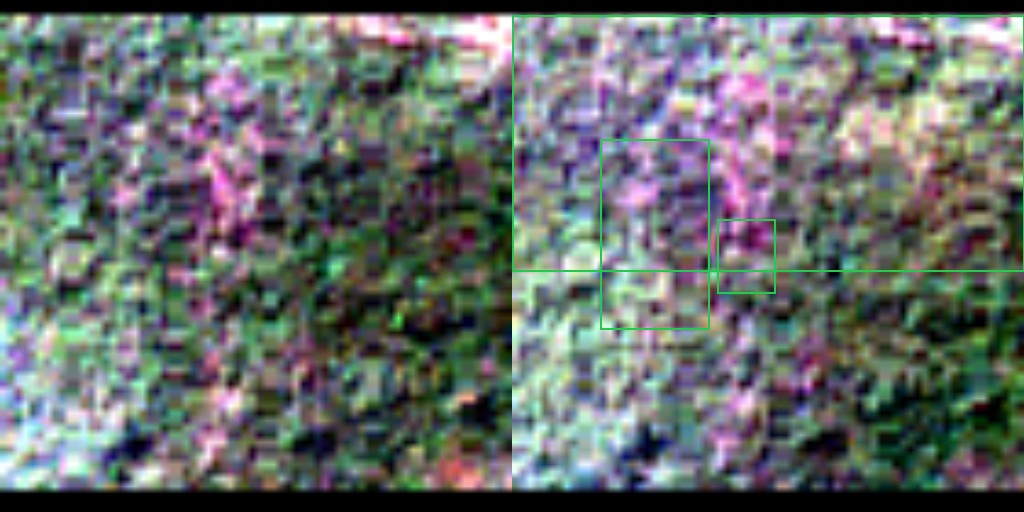
\includegraphics[width=0.72\textwidth]{figures/fig_otsu_p01289.jpg}
\caption{Otsu boxes for p01289 on the T0 (left) and T1 (right) chips, from \file{data/qa_figures/_spotcheck/}. This spot-check was made before the colour fix, so it still shows the purple stretch.}
\label{fig:otsu}
\end{figure}

\begin{watchout}
The September slides describe ``explanations tied to bounding boxes'', but in the final dataset the boxes play almost no role, and the models were never asked about them. The intended rule was probably ``remove boxes when the person says stable or increase''; treating an empty label the same way was a side effect. In the report, mention the boxes briefly as an implemented step that ended up covering three patches, or leave them out.
\end{watchout}

\subsection{What is saved}

\begin{itemize}
  \item Colour canvases as JPEG, quality 95: \file{data/processed_images/pXXXXX_T0.jpg} and \file{_T1.jpg}.
  \item Physical layers as NumPy arrays (\texttt{.npy}), 13 per patch (optical bands, indices, radar, rainfall and ERA5 for both years, terrain, \dndvi, \dnbr), and the Otsu masks in \file{data/evidence_masks/}.
  \item A record of all triplets in \file{data/raw_metadata/triplets.json}.
\end{itemize}

\begin{foryourreport}
In ``Preprocessing and Patch Generation'' (about 450 words):
\begin{itemize}
  \item The candidate pool (1,200), the patch geometry (320\,m circle $\rightarrow$ square $\rightarrow$ clipped to the rectangle), and the export in degrees (about 70\,$\times$\,65 pixels).
  \item The 15 layers per patch (Table~\ref{tab:15files} can go in an appendix).
  \item The masked-fraction filter (0.15) and the very low missing data.
  \item Padding to a square and resizing to 512\,$\times$\,512, saying that this enlarges the chips about seven times and adds no detail.
  \item Otsu, boxes and the policy in two or three sentences at most, since only three patches kept boxes. Equation~\ref{eq:otsu} is optional.
\end{itemize}
Avoid ``the images were downsampled to 512\,$\times$\,512'': they were padded and \emph{enlarged}.
\end{foryourreport}

\begin{selfcheck}
\begin{enumerate}
  \item Why did the ``64\,$\times$\,64'' patches come out as about 70\,$\times$\,65 pixels?
  \item Why is the masked fraction probably not a cloud measurement?
  \item What does padding with zeros do to the averages written into the evidence card?
  \item In one sentence, what does Otsu's method choose?
  \item Why do only three patches have bounding boxes?
\end{enumerate}
\end{selfcheck}
